% ---------------------------------------------------------------------
% CAOS_LDA_HSI series, paper P4: preprint (target venue redacted)
%
% Title  : Which Backbone Picks Which Wordification? A Factorial Study
%          of Topic-Model Families on Hyperspectral Imagery
% Target : redacted while the preprint circulates
% Class  : IEEEtran journal option
% Scope  : LDA, HDP, ProdLDA and ETM over the V1..V20 design space; the
%          canonical equation set is \input from
%          ../../equations/canonical.tex.
% ---------------------------------------------------------------------

\documentclass[journal,a4paper,10pt]{IEEEtran}

\usepackage[utf8]{inputenc}
\usepackage[T1]{fontenc}
\usepackage{amsmath,amssymb,amsfonts}
\usepackage{dsfont}% \mathds{1}: indicator function in the canonical equation set
\usepackage{graphicx}
\usepackage{booktabs}
\usepackage{array}
\usepackage{multirow}
\usepackage{cite}
\usepackage{xcolor}
\usepackage{url}
\usepackage[hidelinks]{hyperref}

\graphicspath{{../../figures/}}

% IEEEtran hard-codes an em-dash after the abstract and index-terms names; the CAOS
% content standard (ADR-0067) excludes em-dashes, so the separator is a full stop.
\makeatletter
\def\abstract{\normalfont
    \if@twocolumn
      \@IEEEabskeysecsize\bfseries\textit{\abstractname}.\ \relax
    \else
      \bgroup\par\addvspace{0.5\baselineskip}\centering\vspace{-1.78ex}\@IEEEabskeysecsize\textbf{\abstractname}\par\addvspace{0.5\baselineskip}\egroup\quotation\@IEEEabskeysecsize
    \fi\@IEEEgobbleleadPARNLSP}
\def\IEEEkeywords{\normalfont
    \if@twocolumn
      \@IEEEabskeysecsize\bfseries\textit{\IEEEkeywordsname}.\ \relax
    \else
      \bgroup\par\addvspace{0.5\baselineskip}\centering\@IEEEabskeysecsize\textbf{\IEEEkeywordsname}\par\addvspace{0.5\baselineskip}\egroup\quotation\@IEEEabskeysecsize
    \fi\@IEEEgobbleleadPARNLSP}
\makeatother

% Page-1 header block (conventions/manuscript-header-standard.md). The four document
% macros are set by the publishing tool when the version DOI is reserved.
\newcommand{\doctype}{Preprint}
\newcommand{\docversion}{v1.5}
\newcommand{\docdate}{19 September 2026}
\newcommand{\versiondoi}{10.5281/zenodo.22850111}
\newcommand{\conceptdoi}{10.5281/zenodo.21504111}
\newcommand{\docrepo}{github.com/fsantibanezleal/CAOS\_LDA\_HSI}
\newcommand{\headerblock}{%
\begin{center}
\fbox{\parbox{0.94\textwidth}{\small\raggedright
\textbf{\doctype} \quad$\cdot$\quad \docversion, \docdate \quad$\cdot$\quad Licence CC BY 4.0\\[2pt]
CAOS open-research programme \quad$\cdot$\quad CAOS\_LDA\_HSI, topic models on hyperspectral imagery (paper P4)\\[2pt]
Version DOI \href{https://doi.org/\versiondoi}{\texttt{\versiondoi}} \quad$\cdot$\quad
concept DOI (always latest) \href{https://doi.org/\conceptdoi}{\texttt{\conceptdoi}}\\[2pt]
Not peer reviewed. Source code, data and computational records: \href{https://\docrepo}{\texttt{\docrepo}}
}}
\end{center}}

\title{Which Backbone Picks Which Wordification? A Factorial Study of
Topic-Model Families on Hyperspectral Imagery}

\author{%
  Felipe Santib\'a\~nez-Leal~\orcidlink{0000-0002-0150-3246},~\IEEEmembership{Independent Researcher}%
  \thanks{F.\ Santib\'a\~nez-Leal is with the CAOS open-research
    programme, Santiago, Chile
    (e-mail: \texttt{fsantibanezleal@ug.uchile.cl};
    ORCID: 0000-0002-0150-3246).}%
  \thanks{Companion papers: \emph{Beyond
    Accuracy}~\cite{santibanezleal2026framework} (P1, twelve-axis
    framework) and \emph{Which Wordification
    Matters?}~\cite{santibanezleal2026sweep} (P3, 19-recipe sweep under
    a fixed LDA backbone). Code and derived artefacts at
    \url{https://github.com/fsantibanezleal/CAOS_LDA_HSI}.}%
  \thanks{This work has been partially funded by AMTC Basal
    (ANID/PIA AFB220002) and ANID FONDECYT Postdoctorado 3220094.}%
}

\markboth{\doctype\ \docversion, 2026 \textperiodcentered\ CAOS open-research programme}{Santib\'a\~nez-Leal:
Backbone $\times$ Wordification Factorial on HSI}

\IEEEaftertitletext{\vspace{-0.6\baselineskip}\headerblock\vspace{0.2\baselineskip}}

\IEEEtitleabstractindextext{%
\begin{abstract}
The companion paper~\cite{santibanezleal2026sweep} showed that nineteen wordification recipes
(V1--V15, V17--V20) produce measurably different topic bases under a
fixed LDA backbone, with no universal winner: V12 (Gaussian-mixture
tokens) has the highest mean coherence and topic--label coupling
(winning two of six scenes on each), V20 (mutual-information-weighted
bands) has the highest counterfactual robustness F-22, and V1 (band-frequency
tokens, the canonical) is the most reliable of the per-band recipes
under reseeding, while F-1 macro-F1 separates the recipes by less than
0.01. This paper asks the orthogonal
question: \emph{does the recipe winner depend on the topic-model
backbone?} We run the full V1--V20 sweep (nineteen recipes; V16 is
scaffolded only) under three additional backbones, namely the
Hierarchical Dirichlet Process (HDP, nonparametric K), the amortised
neural topic model labelled ProdLDA (run in its mixture-decoder form,
with a standard logistic-normal prior) and the Embedded Topic Model
(ETM, the same prior and encoder with a word--topic embedding
decoder), producing a
$4 \times 19$ factorial on six labelled-scene benchmarks
(456 cells in the headline F-2 coherence axis). The headline finding
is that \textbf{the wordification ranking inverts across backbones}.
LDA and ETM agree that V12 wins, HDP picks V7 (absorption-feature
triplets) and ProdLDA picks V3 (joint (band, bin) vocabulary). ETM
and ProdLDA differ only in the decoder parameterisation, so their
different winners come from the decoder or from optimisation; the runs
do not separate the two. We give a per-recipe \emph{affinity score}
that quantifies how each recipe transfers across backbones, identify
three empirical backbone--recipe pairings, and recommend reporting the
$(\text{backbone}, \text{wordification})$ pair as a single hyper-decision
in any future LDA-on-HSI work. LDVAE-T, a Dirichlet-prior unmixing VAE,
is a candidate fifth backbone; it is not evaluated because no public
implementation is available.
\end{abstract}

\begin{IEEEkeywords}
hyperspectral imagery, latent Dirichlet allocation, ProdLDA, ETM, HDP,
wordification, topic models, factorial study, evaluation framework,
backbone choice, learned tokenisation.
\end{IEEEkeywords}}

\usepackage[hidelinks]{hyperref}
\usepackage{orcidlink}

\begin{document}
\bstctlcite{IEEEexample:BSTcontrol}

\maketitle
\IEEEdisplaynontitleabstractindextext
\IEEEpeerreviewmaketitle

% Canonical equation set (single source of truth, shared across P3/P4/P5).
% Do not re-derive: \input here and \eqref the labels below. Unused groups
% (B-recipes other than the four we cite, most of group C) simply go
% un-\eqref'd; they are still typeset but unreferenced.
% ===================================================================
% CANONICAL EQUATION SET: CAOS_LDA_HSI manuscript series (P3/P4/P5)
% ===================================================================
% Single source of truth for all display equations. Authored once,
% \input into P3 (journal_v_sweep), P4 (journal_backbone_factorial),
% P5 (journal_interpretability), and transcribed (KaTeX) into the
% web-app methodology route and the wiki Mathematical-Background page.
%
% Usage:  % ===================================================================
% CANONICAL EQUATION SET: CAOS_LDA_HSI manuscript series (P3/P4/P5)
% ===================================================================
% Single source of truth for all display equations. Authored once,
% \input into P3 (journal_v_sweep), P4 (journal_backbone_factorial),
% P5 (journal_interpretability), and transcribed (KaTeX) into the
% web-app methodology route and the wiki Mathematical-Background page.
%
% Usage:  % ===================================================================
% CANONICAL EQUATION SET: CAOS_LDA_HSI manuscript series (P3/P4/P5)
% ===================================================================
% Single source of truth for all display equations. Authored once,
% \input into P3 (journal_v_sweep), P4 (journal_backbone_factorial),
% P5 (journal_interpretability), and transcribed (KaTeX) into the
% web-app methodology route and the wiki Mathematical-Background page.
%
% Usage:  \input{../../equations/canonical.tex}  then reference the
% groups by \eqref{eq:lda-gen}, \eqref{eq:etm-beta}, etc. Groups can
% also be copied verbatim into a single \begin{align} if a paper wants
% them inline. Each equation is independently labelled.
%
% NOTATION (fixed once, used everywhere):
%   b in {1..B}    spectral band            (B ~ 200)
%   q in {0..Q-1}  quantisation level       (Q in {8,16,32}, default 8)
%   k in {1..K}    topic                    (K per-scene K-policy)
%   d in {1..D}    document = labelled pixel
%   v in V         wordification vocabulary (recipe-specific)
%   x_d in R^B     normalised pixel spectrum
%   y_d            land-cover / mineral label of pixel d
%   theta_d        per-doc topic proportions  (simplex Delta^{K-1})
%   phi_k          topic-word distribution    (simplex Delta^{|V|-1})
%   n_d in N^{|V|} doc-term count vector produced by a recipe
% ===================================================================

% ----- GROUP A : the four topic-model backbones -------------------

% A1  LDA (online variational Bayes; P1/P3 baseline)
\begin{equation}\label{eq:lda-gen}
\begin{gathered}
\phi_k \sim \mathrm{Dir}(\beta),\quad
\theta_d \sim \mathrm{Dir}(\alpha),\\
z_{dn} \sim \mathrm{Cat}(\theta_d),\quad
w_{dn} \sim \mathrm{Cat}(\phi_{z_{dn}}).
\end{gathered}
\end{equation}

% A2  HDP (nonparametric K via two-level stick-breaking)
\begin{equation}\label{eq:hdp-gen}
\begin{gathered}
\boldsymbol{\beta}\sim\mathrm{GEM}(\gamma),\quad
\pi_d \sim \mathrm{DP}(\alpha_0,\boldsymbol{\beta}),\\
z_{dn}\sim\mathrm{Cat}(\pi_d),\quad
w_{dn}\sim\mathrm{Cat}(\phi_{z_{dn}}),
\end{gathered}
\end{equation}
with global atom weights $\beta_k=\beta'_k\prod_{l<k}(1-\beta'_l)$,
$\beta'_k\sim\mathrm{Beta}(1,\gamma)$.

% A3  "ProdLDA" as run: the amortised neural topic model of Srivastava and Sutton
%     in its mixture-decoder form (their NVLDA), with a standard normal prior on
%     the topic-proportion logits delta_d and a free matrix of unnormalised
%     topic-word logits omega_k (no product of experts, no Laplace approximation)
\begin{equation}\label{eq:prodlda-gen}
\begin{gathered}
\delta_d \sim \mathcal{N}(0, I),\quad
\theta_d = \mathrm{softmax}(\delta_d),\\
\beta_k = \mathrm{softmax}(\omega_k),\quad
w_{dn} \sim \mathrm{Cat}\!\Big(\textstyle\sum_k \theta_{dk}\,\beta_k\Big),
\end{gathered}
\end{equation}
where the unnormalised topic--word logits $\omega_k\in\mathbb{R}^{|V|}$ form
a free $K\times|V|$ matrix and inference is amortised,
$(\mu_d,\Sigma_d)=\mathrm{Enc}_\eta(n_d)$. ProdLDA as published mixes the
logits instead, $w_{dn}\sim\mathrm{Cat}\big(\mathrm{softmax}(\textstyle\sum_k \theta_{dk}\,\omega_k)\big)$
(a product of experts), with a Laplace approximation to $\mathrm{Dir}(\alpha)$
as the prior; that form was not run.

% A4  ETM (embedded topic model; same prior and encoder as A3, rank-L decoder)
\begin{equation}\label{eq:etm-beta}
\begin{gathered}
\delta_d \sim \mathcal{N}(0, I),\quad
\theta_d = \mathrm{softmax}(\delta_d),\\
\beta_k = \mathrm{softmax}\!\big(\rho^{\top}\alpha_k\big),\quad
w_{dn}\sim\mathrm{Cat}\!\Big(\textstyle\sum_k \theta_{dk}\,\beta_k\Big),
\end{gathered}
\end{equation}
with word embeddings $\rho\in\mathbb{R}^{L\times|V|}$ and topic
embeddings $\alpha_k\in\mathbb{R}^{L}$ ($L=64$), and the same amortised
encoder as \eqref{eq:prodlda-gen}.

% ----- GROUP B : wordification recipes (spectrum -> doc-term) ------

% B0  per-row min-max normalisation + uniform quantiser
\begin{equation}\label{eq:quantiser}
\begin{gathered}
\tilde{x}_{db}=\frac{x_{db}-\min_b x_{db}}{\max_b x_{db}-\min_b x_{db}},
\\
q_b(x_d)=\mathrm{clip}\big(\lfloor \tilde{x}_{db}\,Q\rfloor,\,0,\,Q-1\big).
\end{gathered}
\end{equation}

% B1  V1 band-frequency: token = band, multiplicity = quantised intensity
\begin{equation}\label{eq:v1}
n_d^{\mathrm{V1}}[b] = q_b(x_d),\qquad |V_{\mathrm{V1}}| = B.
\end{equation}

% B2  V3 joint (band, bin): one token per band naming its bin
\begin{equation}\label{eq:v3}
n_d^{\mathrm{V3}}[(b,q)] = \mathds{1}\!\left[q_b(x_d)=q\right],\qquad
|V_{\mathrm{V3}}| = B\,Q .
\end{equation}

% B3  V8 NFINDR endmember-fraction: FCLS abundances, rescaled by the pixel's largest abundance and
%     quantised to Q levels (build_wordifications_v6plus.wordify_v8_endmember_fraction)
\begin{equation}\label{eq:v8}
\begin{gathered}
a_d=\arg\min_{a\ge 0,\;\mathbf{1}^{\top}a=1}\;\lVert x_d - E\,a\rVert_2^2,\\
n_d^{\mathrm{V8}}[m]=\min\!\Big(\Big\lfloor Q\,\frac{a_{dm}}{\max_{m'} a_{dm'}}\Big\rfloor,\;Q-1\Big),
\end{gathered}
\end{equation}
where $E=[e_1,\dots,e_M]$ are the NFINDR endmembers (simplex vertices),
$x_d$ is the unnormalised spectrum and $|V_{\mathrm{V8}}|=M$. The abundance
non-negativity (ANC, $a\ge 0$) and sum-to-one (ASC, $\mathbf{1}^{\top}a=1$)
constraints make $a_d$ a point on the simplex spanned by the endmembers
(fully-constrained least squares, FCLS; implemented as
$\delta$-augmented NNLS followed by renormalisation), so the coefficients
are proper abundance fractions over the convex hull. The dominant
endmember of every pixel emits $Q-1$ tokens, so the document length
grows with $Q$.

% B4  V12 GMM-token: (band, component) joints from one 1-D Q-component Gaussian mixture fitted to the
%     band intensities (build_wordifications_v6plus.wordify_v12_gmm; hard assignment, not responsibilities)
\begin{equation}\label{eq:v12}
\begin{gathered}
g_b(x_d)=\arg\max_{k\in\{0,\dots,Q-1\}}\;\pi_k\,\mathcal{N}\big(x_{db}\mid\mu_k,\sigma_k^2\big),\\
n_d^{\mathrm{V12}}[(b,g)]=\mathds{1}\!\left[g_b(x_d)=g\right],\qquad
|V_{\mathrm{V12}}|=B\,Q,
\end{gathered}
\end{equation}
where $(\pi_k,\mu_k,\sigma_k^2)_{k<Q}$ is a one-dimensional Gaussian
mixture fitted once per scene to the unnormalised band intensities of the
sampled pixels (a random subset of 50\,000 values), with the components
indexed in increasing order of $\mu_k$. Each band emits one token, as in
V3, but the bins are shared by all pixels and follow the intensity
distribution instead of splitting each spectrum's own range into equal
intervals.

% B5  V20 MI-weighted bands: V3 alphabet, per-band emission multiplicity
\begin{equation}\label{eq:v20}
\begin{gathered}
w_b=\Big\lfloor \tfrac{\mathrm{MI}(x_{\cdot b};\,y)}{\max_{b'}\mathrm{MI}(x_{\cdot b'};\,y)}\;Q_{\max}\Big\rceil,
\\
n_d^{\mathrm{V20}}[(b,q)] = w_b\,\mathds{1}\!\left[q_b(x_d)=q\right].
\end{gathered}
\end{equation}
The token alphabet is V3's, $|V_{\mathrm{V20}}|=B\,Q$ (=1600 at
$B=200,Q=8$; mean $\approx 1376$ across the six labelled scenes since
$B$ varies). Bands with $w_b=0$ emit nothing, so the \emph{effective}
(non-empty-column) vocabulary is smaller still ($\approx 770$ mean).

% ----- GROUP C : evaluation axes ----------------------------------

% C1  F-1 macro-F1 (5-fold; topic_routed_soft head)
\begin{equation}\label{eq:f1}
\mathrm{F\text{-}1}=\frac{1}{|\mathcal{C}|}\sum_{c\in\mathcal{C}}
\frac{2\,P_c R_c}{P_c+R_c}.
\end{equation}

% C2  F-2 coherence c_v (NPMI sliding window + cosine aggregation)
\begin{equation}\label{eq:f2}
\begin{gathered}
\mathrm{NPMI}(w_i,w_j)=\frac{\log\frac{p(w_i,w_j)+\epsilon}{p(w_i)p(w_j)}}{-\log\big(p(w_i,w_j)+\epsilon\big)},\\
c_v=\frac{1}{N}\sum_{i}\cos\!\big(\mathbf{v}_i,\,\textstyle\sum_j \mathbf{v}_j\big),
\end{gathered}
\end{equation}
with $\mathbf{v}_i=\big(\mathrm{NPMI}(w_i,w_\ell)\big)_{\ell=1}^{N}$ over the
top-$N$ topic words.

% C3  F-7 topic-to-label MI normalised by H(label) -- this is the
% ASYMMETRIC label-normalised MI (uncertainty coefficient U(Y|Zhat) =
% completeness, Rosenberg-Hirschberg 2007), NOT the symmetric NMI
% I/sqrt(H H). Uncorrected for chance.
\begin{equation}\label{eq:f7}
\begin{gathered}
\hat{z}_d=\arg\max_k \theta_{dk},\\
\mathrm{F\text{-}7}=\frac{I(\hat{Z};Y)}{H(Y)}
\;=\; U(Y\mid\hat{Z})\;=\;1-\frac{H(Y\mid\hat{Z})}{H(Y)}.
\end{gathered}
\end{equation}

% C4  F-14 top-N pairwise Jaccard repetitiveness (lower = more diverse)
\begin{equation}\label{eq:f14}
\mathrm{F\text{-}14}=\frac{2}{K(K-1)}\sum_{k<k'}
\frac{|T_k\cap T_{k'}|}{|T_k\cup T_{k'}|},\qquad T_k=\text{top-}N(\phi_k).
\end{equation}

% C5  F-18 Maier reseed reliability (Hungarian-matched top-N cosine)
\begin{equation}\label{eq:f18}
\mathrm{F\text{-}18}=\frac{1}{\binom{S}{2}}\sum_{s<s'}\frac{1}{K}
\max_{\sigma\in\mathfrak{S}_K}\sum_{k}\cos\!\big(\mathbf{u}^{(s)}_k,\mathbf{u}^{(s')}_{\sigma(k)}\big),
\end{equation}
over $S$ reseeded refits, with $\mathbf{u}^{(s)}_k$ the top-$N$ indicator
vector of topic $k$ in run $s$.

% C6  F-22 counterfactual L1 (min token perturbation to flip argmax topic)
\begin{equation}\label{eq:f22}
\begin{aligned}
\mathrm{F\text{-}22}(d)={}&\min_{\delta\in\mathbb{Z}^{|V|}}\lVert\delta\rVert_1
\;\;\text{s.t.}\\
&\arg\max_k\theta_k(n_d+\delta)\neq\arg\max_k\theta_k(n_d),\\
&n_d+\delta\ge 0,
\end{aligned}
\end{equation}
reported as the per-scene median, capped at a sentinel
$\mathrm{MAX\_STEPS}=50$ when no flip is found.

% C7  F-15 LLM-judge alignment (top-N overlap rule, as the judge implementation computes it:
%     ambiguous documents, i.e. neither aligned nor with >= 3 non-zero tokens, are excluded)
\begin{equation}\label{eq:f15}
\begin{aligned}
\mathrm{aligned}(d)&=\mathds{1}\big[\,|\mathrm{top}_N(n_d)\cap\mathrm{top}_N(\phi_{\hat{z}_d})|\ge\tau\\
&\qquad\;\vee\;\mathrm{top}_3(n_d)\cap\mathrm{top}_N(\phi_{\hat{z}_d})\neq\emptyset\,\big],\\
\mathrm{decisive}(d)&=\mathds{1}\big[\,\mathrm{aligned}(d)=1\;\vee\;|\mathrm{supp}(n_d)|\ge 3\,\big],\\
\mathrm{F\text{-}15}&=\textstyle\sum_d \mathrm{aligned}(d)\,\big/\textstyle\sum_d \mathrm{decisive}(d).
\end{aligned}
\end{equation}

% C8  token-mass dispersion (P5 mechanism metric: effective vocabulary)
\begin{equation}\label{eq:dispersion}
\begin{gathered}
p_{dv}=\frac{n_{dv}}{\sum_{v'} n_{dv'}},\\
N_{\mathrm{eff}}(d)=\exp\!\big(H(p_d)\big)=\exp\!\Big(-\sum_v p_{dv}\log p_{dv}\Big).
\end{gathered}
\end{equation}
$N_{\mathrm{eff}}$ counts the tokens that effectively carry the mass of
$p_d$ (or of a topic's $\phi_k$): it is low when the mass is concentrated
on few tokens and at most $|V|$.

% ----- GROUP D : cross-backbone affinity score (P4) ----------------

% D1  per-recipe cross-backbone affinity (min-max normalised within backbone)
\begin{equation}\label{eq:affinity}
\mathcal{A}(V_i)=\frac{1}{|\mathcal{B}|}\sum_{m\in\mathcal{B}}
\frac{c_v^{(m)}(V_i)-\min_j c_v^{(m)}(V_j)}{\max_j c_v^{(m)}(V_j)-\min_j c_v^{(m)}(V_j)}\;\in[0,1],
\end{equation}
averaged over backbones $\mathcal{B}=\{\mathrm{LDA},\mathrm{HDP},\mathrm{ProdLDA},\mathrm{ETM}\}$;
$\mathcal{A}\to 1$ when a recipe sits near the per-backbone top everywhere.
  then reference the
% groups by \eqref{eq:lda-gen}, \eqref{eq:etm-beta}, etc. Groups can
% also be copied verbatim into a single \begin{align} if a paper wants
% them inline. Each equation is independently labelled.
%
% NOTATION (fixed once, used everywhere):
%   b in {1..B}    spectral band            (B ~ 200)
%   q in {0..Q-1}  quantisation level       (Q in {8,16,32}, default 8)
%   k in {1..K}    topic                    (K per-scene K-policy)
%   d in {1..D}    document = labelled pixel
%   v in V         wordification vocabulary (recipe-specific)
%   x_d in R^B     normalised pixel spectrum
%   y_d            land-cover / mineral label of pixel d
%   theta_d        per-doc topic proportions  (simplex Delta^{K-1})
%   phi_k          topic-word distribution    (simplex Delta^{|V|-1})
%   n_d in N^{|V|} doc-term count vector produced by a recipe
% ===================================================================

% ----- GROUP A : the four topic-model backbones -------------------

% A1  LDA (online variational Bayes; P1/P3 baseline)
\begin{equation}\label{eq:lda-gen}
\begin{gathered}
\phi_k \sim \mathrm{Dir}(\beta),\quad
\theta_d \sim \mathrm{Dir}(\alpha),\\
z_{dn} \sim \mathrm{Cat}(\theta_d),\quad
w_{dn} \sim \mathrm{Cat}(\phi_{z_{dn}}).
\end{gathered}
\end{equation}

% A2  HDP (nonparametric K via two-level stick-breaking)
\begin{equation}\label{eq:hdp-gen}
\begin{gathered}
\boldsymbol{\beta}\sim\mathrm{GEM}(\gamma),\quad
\pi_d \sim \mathrm{DP}(\alpha_0,\boldsymbol{\beta}),\\
z_{dn}\sim\mathrm{Cat}(\pi_d),\quad
w_{dn}\sim\mathrm{Cat}(\phi_{z_{dn}}),
\end{gathered}
\end{equation}
with global atom weights $\beta_k=\beta'_k\prod_{l<k}(1-\beta'_l)$,
$\beta'_k\sim\mathrm{Beta}(1,\gamma)$.

% A3  "ProdLDA" as run: the amortised neural topic model of Srivastava and Sutton
%     in its mixture-decoder form (their NVLDA), with a standard normal prior on
%     the topic-proportion logits delta_d and a free matrix of unnormalised
%     topic-word logits omega_k (no product of experts, no Laplace approximation)
\begin{equation}\label{eq:prodlda-gen}
\begin{gathered}
\delta_d \sim \mathcal{N}(0, I),\quad
\theta_d = \mathrm{softmax}(\delta_d),\\
\beta_k = \mathrm{softmax}(\omega_k),\quad
w_{dn} \sim \mathrm{Cat}\!\Big(\textstyle\sum_k \theta_{dk}\,\beta_k\Big),
\end{gathered}
\end{equation}
where the unnormalised topic--word logits $\omega_k\in\mathbb{R}^{|V|}$ form
a free $K\times|V|$ matrix and inference is amortised,
$(\mu_d,\Sigma_d)=\mathrm{Enc}_\eta(n_d)$. ProdLDA as published mixes the
logits instead, $w_{dn}\sim\mathrm{Cat}\big(\mathrm{softmax}(\textstyle\sum_k \theta_{dk}\,\omega_k)\big)$
(a product of experts), with a Laplace approximation to $\mathrm{Dir}(\alpha)$
as the prior; that form was not run.

% A4  ETM (embedded topic model; same prior and encoder as A3, rank-L decoder)
\begin{equation}\label{eq:etm-beta}
\begin{gathered}
\delta_d \sim \mathcal{N}(0, I),\quad
\theta_d = \mathrm{softmax}(\delta_d),\\
\beta_k = \mathrm{softmax}\!\big(\rho^{\top}\alpha_k\big),\quad
w_{dn}\sim\mathrm{Cat}\!\Big(\textstyle\sum_k \theta_{dk}\,\beta_k\Big),
\end{gathered}
\end{equation}
with word embeddings $\rho\in\mathbb{R}^{L\times|V|}$ and topic
embeddings $\alpha_k\in\mathbb{R}^{L}$ ($L=64$), and the same amortised
encoder as \eqref{eq:prodlda-gen}.

% ----- GROUP B : wordification recipes (spectrum -> doc-term) ------

% B0  per-row min-max normalisation + uniform quantiser
\begin{equation}\label{eq:quantiser}
\begin{gathered}
\tilde{x}_{db}=\frac{x_{db}-\min_b x_{db}}{\max_b x_{db}-\min_b x_{db}},
\\
q_b(x_d)=\mathrm{clip}\big(\lfloor \tilde{x}_{db}\,Q\rfloor,\,0,\,Q-1\big).
\end{gathered}
\end{equation}

% B1  V1 band-frequency: token = band, multiplicity = quantised intensity
\begin{equation}\label{eq:v1}
n_d^{\mathrm{V1}}[b] = q_b(x_d),\qquad |V_{\mathrm{V1}}| = B.
\end{equation}

% B2  V3 joint (band, bin): one token per band naming its bin
\begin{equation}\label{eq:v3}
n_d^{\mathrm{V3}}[(b,q)] = \mathds{1}\!\left[q_b(x_d)=q\right],\qquad
|V_{\mathrm{V3}}| = B\,Q .
\end{equation}

% B3  V8 NFINDR endmember-fraction: FCLS abundances, rescaled by the pixel's largest abundance and
%     quantised to Q levels (build_wordifications_v6plus.wordify_v8_endmember_fraction)
\begin{equation}\label{eq:v8}
\begin{gathered}
a_d=\arg\min_{a\ge 0,\;\mathbf{1}^{\top}a=1}\;\lVert x_d - E\,a\rVert_2^2,\\
n_d^{\mathrm{V8}}[m]=\min\!\Big(\Big\lfloor Q\,\frac{a_{dm}}{\max_{m'} a_{dm'}}\Big\rfloor,\;Q-1\Big),
\end{gathered}
\end{equation}
where $E=[e_1,\dots,e_M]$ are the NFINDR endmembers (simplex vertices),
$x_d$ is the unnormalised spectrum and $|V_{\mathrm{V8}}|=M$. The abundance
non-negativity (ANC, $a\ge 0$) and sum-to-one (ASC, $\mathbf{1}^{\top}a=1$)
constraints make $a_d$ a point on the simplex spanned by the endmembers
(fully-constrained least squares, FCLS; implemented as
$\delta$-augmented NNLS followed by renormalisation), so the coefficients
are proper abundance fractions over the convex hull. The dominant
endmember of every pixel emits $Q-1$ tokens, so the document length
grows with $Q$.

% B4  V12 GMM-token: (band, component) joints from one 1-D Q-component Gaussian mixture fitted to the
%     band intensities (build_wordifications_v6plus.wordify_v12_gmm; hard assignment, not responsibilities)
\begin{equation}\label{eq:v12}
\begin{gathered}
g_b(x_d)=\arg\max_{k\in\{0,\dots,Q-1\}}\;\pi_k\,\mathcal{N}\big(x_{db}\mid\mu_k,\sigma_k^2\big),\\
n_d^{\mathrm{V12}}[(b,g)]=\mathds{1}\!\left[g_b(x_d)=g\right],\qquad
|V_{\mathrm{V12}}|=B\,Q,
\end{gathered}
\end{equation}
where $(\pi_k,\mu_k,\sigma_k^2)_{k<Q}$ is a one-dimensional Gaussian
mixture fitted once per scene to the unnormalised band intensities of the
sampled pixels (a random subset of 50\,000 values), with the components
indexed in increasing order of $\mu_k$. Each band emits one token, as in
V3, but the bins are shared by all pixels and follow the intensity
distribution instead of splitting each spectrum's own range into equal
intervals.

% B5  V20 MI-weighted bands: V3 alphabet, per-band emission multiplicity
\begin{equation}\label{eq:v20}
\begin{gathered}
w_b=\Big\lfloor \tfrac{\mathrm{MI}(x_{\cdot b};\,y)}{\max_{b'}\mathrm{MI}(x_{\cdot b'};\,y)}\;Q_{\max}\Big\rceil,
\\
n_d^{\mathrm{V20}}[(b,q)] = w_b\,\mathds{1}\!\left[q_b(x_d)=q\right].
\end{gathered}
\end{equation}
The token alphabet is V3's, $|V_{\mathrm{V20}}|=B\,Q$ (=1600 at
$B=200,Q=8$; mean $\approx 1376$ across the six labelled scenes since
$B$ varies). Bands with $w_b=0$ emit nothing, so the \emph{effective}
(non-empty-column) vocabulary is smaller still ($\approx 770$ mean).

% ----- GROUP C : evaluation axes ----------------------------------

% C1  F-1 macro-F1 (5-fold; topic_routed_soft head)
\begin{equation}\label{eq:f1}
\mathrm{F\text{-}1}=\frac{1}{|\mathcal{C}|}\sum_{c\in\mathcal{C}}
\frac{2\,P_c R_c}{P_c+R_c}.
\end{equation}

% C2  F-2 coherence c_v (NPMI sliding window + cosine aggregation)
\begin{equation}\label{eq:f2}
\begin{gathered}
\mathrm{NPMI}(w_i,w_j)=\frac{\log\frac{p(w_i,w_j)+\epsilon}{p(w_i)p(w_j)}}{-\log\big(p(w_i,w_j)+\epsilon\big)},\\
c_v=\frac{1}{N}\sum_{i}\cos\!\big(\mathbf{v}_i,\,\textstyle\sum_j \mathbf{v}_j\big),
\end{gathered}
\end{equation}
with $\mathbf{v}_i=\big(\mathrm{NPMI}(w_i,w_\ell)\big)_{\ell=1}^{N}$ over the
top-$N$ topic words.

% C3  F-7 topic-to-label MI normalised by H(label) -- this is the
% ASYMMETRIC label-normalised MI (uncertainty coefficient U(Y|Zhat) =
% completeness, Rosenberg-Hirschberg 2007), NOT the symmetric NMI
% I/sqrt(H H). Uncorrected for chance.
\begin{equation}\label{eq:f7}
\begin{gathered}
\hat{z}_d=\arg\max_k \theta_{dk},\\
\mathrm{F\text{-}7}=\frac{I(\hat{Z};Y)}{H(Y)}
\;=\; U(Y\mid\hat{Z})\;=\;1-\frac{H(Y\mid\hat{Z})}{H(Y)}.
\end{gathered}
\end{equation}

% C4  F-14 top-N pairwise Jaccard repetitiveness (lower = more diverse)
\begin{equation}\label{eq:f14}
\mathrm{F\text{-}14}=\frac{2}{K(K-1)}\sum_{k<k'}
\frac{|T_k\cap T_{k'}|}{|T_k\cup T_{k'}|},\qquad T_k=\text{top-}N(\phi_k).
\end{equation}

% C5  F-18 Maier reseed reliability (Hungarian-matched top-N cosine)
\begin{equation}\label{eq:f18}
\mathrm{F\text{-}18}=\frac{1}{\binom{S}{2}}\sum_{s<s'}\frac{1}{K}
\max_{\sigma\in\mathfrak{S}_K}\sum_{k}\cos\!\big(\mathbf{u}^{(s)}_k,\mathbf{u}^{(s')}_{\sigma(k)}\big),
\end{equation}
over $S$ reseeded refits, with $\mathbf{u}^{(s)}_k$ the top-$N$ indicator
vector of topic $k$ in run $s$.

% C6  F-22 counterfactual L1 (min token perturbation to flip argmax topic)
\begin{equation}\label{eq:f22}
\begin{aligned}
\mathrm{F\text{-}22}(d)={}&\min_{\delta\in\mathbb{Z}^{|V|}}\lVert\delta\rVert_1
\;\;\text{s.t.}\\
&\arg\max_k\theta_k(n_d+\delta)\neq\arg\max_k\theta_k(n_d),\\
&n_d+\delta\ge 0,
\end{aligned}
\end{equation}
reported as the per-scene median, capped at a sentinel
$\mathrm{MAX\_STEPS}=50$ when no flip is found.

% C7  F-15 LLM-judge alignment (top-N overlap rule, as the judge implementation computes it:
%     ambiguous documents, i.e. neither aligned nor with >= 3 non-zero tokens, are excluded)
\begin{equation}\label{eq:f15}
\begin{aligned}
\mathrm{aligned}(d)&=\mathds{1}\big[\,|\mathrm{top}_N(n_d)\cap\mathrm{top}_N(\phi_{\hat{z}_d})|\ge\tau\\
&\qquad\;\vee\;\mathrm{top}_3(n_d)\cap\mathrm{top}_N(\phi_{\hat{z}_d})\neq\emptyset\,\big],\\
\mathrm{decisive}(d)&=\mathds{1}\big[\,\mathrm{aligned}(d)=1\;\vee\;|\mathrm{supp}(n_d)|\ge 3\,\big],\\
\mathrm{F\text{-}15}&=\textstyle\sum_d \mathrm{aligned}(d)\,\big/\textstyle\sum_d \mathrm{decisive}(d).
\end{aligned}
\end{equation}

% C8  token-mass dispersion (P5 mechanism metric: effective vocabulary)
\begin{equation}\label{eq:dispersion}
\begin{gathered}
p_{dv}=\frac{n_{dv}}{\sum_{v'} n_{dv'}},\\
N_{\mathrm{eff}}(d)=\exp\!\big(H(p_d)\big)=\exp\!\Big(-\sum_v p_{dv}\log p_{dv}\Big).
\end{gathered}
\end{equation}
$N_{\mathrm{eff}}$ counts the tokens that effectively carry the mass of
$p_d$ (or of a topic's $\phi_k$): it is low when the mass is concentrated
on few tokens and at most $|V|$.

% ----- GROUP D : cross-backbone affinity score (P4) ----------------

% D1  per-recipe cross-backbone affinity (min-max normalised within backbone)
\begin{equation}\label{eq:affinity}
\mathcal{A}(V_i)=\frac{1}{|\mathcal{B}|}\sum_{m\in\mathcal{B}}
\frac{c_v^{(m)}(V_i)-\min_j c_v^{(m)}(V_j)}{\max_j c_v^{(m)}(V_j)-\min_j c_v^{(m)}(V_j)}\;\in[0,1],
\end{equation}
averaged over backbones $\mathcal{B}=\{\mathrm{LDA},\mathrm{HDP},\mathrm{ProdLDA},\mathrm{ETM}\}$;
$\mathcal{A}\to 1$ when a recipe sits near the per-backbone top everywhere.
  then reference the
% groups by \eqref{eq:lda-gen}, \eqref{eq:etm-beta}, etc. Groups can
% also be copied verbatim into a single \begin{align} if a paper wants
% them inline. Each equation is independently labelled.
%
% NOTATION (fixed once, used everywhere):
%   b in {1..B}    spectral band            (B ~ 200)
%   q in {0..Q-1}  quantisation level       (Q in {8,16,32}, default 8)
%   k in {1..K}    topic                    (K per-scene K-policy)
%   d in {1..D}    document = labelled pixel
%   v in V         wordification vocabulary (recipe-specific)
%   x_d in R^B     normalised pixel spectrum
%   y_d            land-cover / mineral label of pixel d
%   theta_d        per-doc topic proportions  (simplex Delta^{K-1})
%   phi_k          topic-word distribution    (simplex Delta^{|V|-1})
%   n_d in N^{|V|} doc-term count vector produced by a recipe
% ===================================================================

% ----- GROUP A : the four topic-model backbones -------------------

% A1  LDA (online variational Bayes; P1/P3 baseline)
\begin{equation}\label{eq:lda-gen}
\begin{gathered}
\phi_k \sim \mathrm{Dir}(\beta),\quad
\theta_d \sim \mathrm{Dir}(\alpha),\\
z_{dn} \sim \mathrm{Cat}(\theta_d),\quad
w_{dn} \sim \mathrm{Cat}(\phi_{z_{dn}}).
\end{gathered}
\end{equation}

% A2  HDP (nonparametric K via two-level stick-breaking)
\begin{equation}\label{eq:hdp-gen}
\begin{gathered}
\boldsymbol{\beta}\sim\mathrm{GEM}(\gamma),\quad
\pi_d \sim \mathrm{DP}(\alpha_0,\boldsymbol{\beta}),\\
z_{dn}\sim\mathrm{Cat}(\pi_d),\quad
w_{dn}\sim\mathrm{Cat}(\phi_{z_{dn}}),
\end{gathered}
\end{equation}
with global atom weights $\beta_k=\beta'_k\prod_{l<k}(1-\beta'_l)$,
$\beta'_k\sim\mathrm{Beta}(1,\gamma)$.

% A3  "ProdLDA" as run: the amortised neural topic model of Srivastava and Sutton
%     in its mixture-decoder form (their NVLDA), with a standard normal prior on
%     the topic-proportion logits delta_d and a free matrix of unnormalised
%     topic-word logits omega_k (no product of experts, no Laplace approximation)
\begin{equation}\label{eq:prodlda-gen}
\begin{gathered}
\delta_d \sim \mathcal{N}(0, I),\quad
\theta_d = \mathrm{softmax}(\delta_d),\\
\beta_k = \mathrm{softmax}(\omega_k),\quad
w_{dn} \sim \mathrm{Cat}\!\Big(\textstyle\sum_k \theta_{dk}\,\beta_k\Big),
\end{gathered}
\end{equation}
where the unnormalised topic--word logits $\omega_k\in\mathbb{R}^{|V|}$ form
a free $K\times|V|$ matrix and inference is amortised,
$(\mu_d,\Sigma_d)=\mathrm{Enc}_\eta(n_d)$. ProdLDA as published mixes the
logits instead, $w_{dn}\sim\mathrm{Cat}\big(\mathrm{softmax}(\textstyle\sum_k \theta_{dk}\,\omega_k)\big)$
(a product of experts), with a Laplace approximation to $\mathrm{Dir}(\alpha)$
as the prior; that form was not run.

% A4  ETM (embedded topic model; same prior and encoder as A3, rank-L decoder)
\begin{equation}\label{eq:etm-beta}
\begin{gathered}
\delta_d \sim \mathcal{N}(0, I),\quad
\theta_d = \mathrm{softmax}(\delta_d),\\
\beta_k = \mathrm{softmax}\!\big(\rho^{\top}\alpha_k\big),\quad
w_{dn}\sim\mathrm{Cat}\!\Big(\textstyle\sum_k \theta_{dk}\,\beta_k\Big),
\end{gathered}
\end{equation}
with word embeddings $\rho\in\mathbb{R}^{L\times|V|}$ and topic
embeddings $\alpha_k\in\mathbb{R}^{L}$ ($L=64$), and the same amortised
encoder as \eqref{eq:prodlda-gen}.

% ----- GROUP B : wordification recipes (spectrum -> doc-term) ------

% B0  per-row min-max normalisation + uniform quantiser
\begin{equation}\label{eq:quantiser}
\begin{gathered}
\tilde{x}_{db}=\frac{x_{db}-\min_b x_{db}}{\max_b x_{db}-\min_b x_{db}},
\\
q_b(x_d)=\mathrm{clip}\big(\lfloor \tilde{x}_{db}\,Q\rfloor,\,0,\,Q-1\big).
\end{gathered}
\end{equation}

% B1  V1 band-frequency: token = band, multiplicity = quantised intensity
\begin{equation}\label{eq:v1}
n_d^{\mathrm{V1}}[b] = q_b(x_d),\qquad |V_{\mathrm{V1}}| = B.
\end{equation}

% B2  V3 joint (band, bin): one token per band naming its bin
\begin{equation}\label{eq:v3}
n_d^{\mathrm{V3}}[(b,q)] = \mathds{1}\!\left[q_b(x_d)=q\right],\qquad
|V_{\mathrm{V3}}| = B\,Q .
\end{equation}

% B3  V8 NFINDR endmember-fraction: FCLS abundances, rescaled by the pixel's largest abundance and
%     quantised to Q levels (build_wordifications_v6plus.wordify_v8_endmember_fraction)
\begin{equation}\label{eq:v8}
\begin{gathered}
a_d=\arg\min_{a\ge 0,\;\mathbf{1}^{\top}a=1}\;\lVert x_d - E\,a\rVert_2^2,\\
n_d^{\mathrm{V8}}[m]=\min\!\Big(\Big\lfloor Q\,\frac{a_{dm}}{\max_{m'} a_{dm'}}\Big\rfloor,\;Q-1\Big),
\end{gathered}
\end{equation}
where $E=[e_1,\dots,e_M]$ are the NFINDR endmembers (simplex vertices),
$x_d$ is the unnormalised spectrum and $|V_{\mathrm{V8}}|=M$. The abundance
non-negativity (ANC, $a\ge 0$) and sum-to-one (ASC, $\mathbf{1}^{\top}a=1$)
constraints make $a_d$ a point on the simplex spanned by the endmembers
(fully-constrained least squares, FCLS; implemented as
$\delta$-augmented NNLS followed by renormalisation), so the coefficients
are proper abundance fractions over the convex hull. The dominant
endmember of every pixel emits $Q-1$ tokens, so the document length
grows with $Q$.

% B4  V12 GMM-token: (band, component) joints from one 1-D Q-component Gaussian mixture fitted to the
%     band intensities (build_wordifications_v6plus.wordify_v12_gmm; hard assignment, not responsibilities)
\begin{equation}\label{eq:v12}
\begin{gathered}
g_b(x_d)=\arg\max_{k\in\{0,\dots,Q-1\}}\;\pi_k\,\mathcal{N}\big(x_{db}\mid\mu_k,\sigma_k^2\big),\\
n_d^{\mathrm{V12}}[(b,g)]=\mathds{1}\!\left[g_b(x_d)=g\right],\qquad
|V_{\mathrm{V12}}|=B\,Q,
\end{gathered}
\end{equation}
where $(\pi_k,\mu_k,\sigma_k^2)_{k<Q}$ is a one-dimensional Gaussian
mixture fitted once per scene to the unnormalised band intensities of the
sampled pixels (a random subset of 50\,000 values), with the components
indexed in increasing order of $\mu_k$. Each band emits one token, as in
V3, but the bins are shared by all pixels and follow the intensity
distribution instead of splitting each spectrum's own range into equal
intervals.

% B5  V20 MI-weighted bands: V3 alphabet, per-band emission multiplicity
\begin{equation}\label{eq:v20}
\begin{gathered}
w_b=\Big\lfloor \tfrac{\mathrm{MI}(x_{\cdot b};\,y)}{\max_{b'}\mathrm{MI}(x_{\cdot b'};\,y)}\;Q_{\max}\Big\rceil,
\\
n_d^{\mathrm{V20}}[(b,q)] = w_b\,\mathds{1}\!\left[q_b(x_d)=q\right].
\end{gathered}
\end{equation}
The token alphabet is V3's, $|V_{\mathrm{V20}}|=B\,Q$ (=1600 at
$B=200,Q=8$; mean $\approx 1376$ across the six labelled scenes since
$B$ varies). Bands with $w_b=0$ emit nothing, so the \emph{effective}
(non-empty-column) vocabulary is smaller still ($\approx 770$ mean).

% ----- GROUP C : evaluation axes ----------------------------------

% C1  F-1 macro-F1 (5-fold; topic_routed_soft head)
\begin{equation}\label{eq:f1}
\mathrm{F\text{-}1}=\frac{1}{|\mathcal{C}|}\sum_{c\in\mathcal{C}}
\frac{2\,P_c R_c}{P_c+R_c}.
\end{equation}

% C2  F-2 coherence c_v (NPMI sliding window + cosine aggregation)
\begin{equation}\label{eq:f2}
\begin{gathered}
\mathrm{NPMI}(w_i,w_j)=\frac{\log\frac{p(w_i,w_j)+\epsilon}{p(w_i)p(w_j)}}{-\log\big(p(w_i,w_j)+\epsilon\big)},\\
c_v=\frac{1}{N}\sum_{i}\cos\!\big(\mathbf{v}_i,\,\textstyle\sum_j \mathbf{v}_j\big),
\end{gathered}
\end{equation}
with $\mathbf{v}_i=\big(\mathrm{NPMI}(w_i,w_\ell)\big)_{\ell=1}^{N}$ over the
top-$N$ topic words.

% C3  F-7 topic-to-label MI normalised by H(label) -- this is the
% ASYMMETRIC label-normalised MI (uncertainty coefficient U(Y|Zhat) =
% completeness, Rosenberg-Hirschberg 2007), NOT the symmetric NMI
% I/sqrt(H H). Uncorrected for chance.
\begin{equation}\label{eq:f7}
\begin{gathered}
\hat{z}_d=\arg\max_k \theta_{dk},\\
\mathrm{F\text{-}7}=\frac{I(\hat{Z};Y)}{H(Y)}
\;=\; U(Y\mid\hat{Z})\;=\;1-\frac{H(Y\mid\hat{Z})}{H(Y)}.
\end{gathered}
\end{equation}

% C4  F-14 top-N pairwise Jaccard repetitiveness (lower = more diverse)
\begin{equation}\label{eq:f14}
\mathrm{F\text{-}14}=\frac{2}{K(K-1)}\sum_{k<k'}
\frac{|T_k\cap T_{k'}|}{|T_k\cup T_{k'}|},\qquad T_k=\text{top-}N(\phi_k).
\end{equation}

% C5  F-18 Maier reseed reliability (Hungarian-matched top-N cosine)
\begin{equation}\label{eq:f18}
\mathrm{F\text{-}18}=\frac{1}{\binom{S}{2}}\sum_{s<s'}\frac{1}{K}
\max_{\sigma\in\mathfrak{S}_K}\sum_{k}\cos\!\big(\mathbf{u}^{(s)}_k,\mathbf{u}^{(s')}_{\sigma(k)}\big),
\end{equation}
over $S$ reseeded refits, with $\mathbf{u}^{(s)}_k$ the top-$N$ indicator
vector of topic $k$ in run $s$.

% C6  F-22 counterfactual L1 (min token perturbation to flip argmax topic)
\begin{equation}\label{eq:f22}
\begin{aligned}
\mathrm{F\text{-}22}(d)={}&\min_{\delta\in\mathbb{Z}^{|V|}}\lVert\delta\rVert_1
\;\;\text{s.t.}\\
&\arg\max_k\theta_k(n_d+\delta)\neq\arg\max_k\theta_k(n_d),\\
&n_d+\delta\ge 0,
\end{aligned}
\end{equation}
reported as the per-scene median, capped at a sentinel
$\mathrm{MAX\_STEPS}=50$ when no flip is found.

% C7  F-15 LLM-judge alignment (top-N overlap rule, as the judge implementation computes it:
%     ambiguous documents, i.e. neither aligned nor with >= 3 non-zero tokens, are excluded)
\begin{equation}\label{eq:f15}
\begin{aligned}
\mathrm{aligned}(d)&=\mathds{1}\big[\,|\mathrm{top}_N(n_d)\cap\mathrm{top}_N(\phi_{\hat{z}_d})|\ge\tau\\
&\qquad\;\vee\;\mathrm{top}_3(n_d)\cap\mathrm{top}_N(\phi_{\hat{z}_d})\neq\emptyset\,\big],\\
\mathrm{decisive}(d)&=\mathds{1}\big[\,\mathrm{aligned}(d)=1\;\vee\;|\mathrm{supp}(n_d)|\ge 3\,\big],\\
\mathrm{F\text{-}15}&=\textstyle\sum_d \mathrm{aligned}(d)\,\big/\textstyle\sum_d \mathrm{decisive}(d).
\end{aligned}
\end{equation}

% C8  token-mass dispersion (P5 mechanism metric: effective vocabulary)
\begin{equation}\label{eq:dispersion}
\begin{gathered}
p_{dv}=\frac{n_{dv}}{\sum_{v'} n_{dv'}},\\
N_{\mathrm{eff}}(d)=\exp\!\big(H(p_d)\big)=\exp\!\Big(-\sum_v p_{dv}\log p_{dv}\Big).
\end{gathered}
\end{equation}
$N_{\mathrm{eff}}$ counts the tokens that effectively carry the mass of
$p_d$ (or of a topic's $\phi_k$): it is low when the mass is concentrated
on few tokens and at most $|V|$.

% ----- GROUP D : cross-backbone affinity score (P4) ----------------

% D1  per-recipe cross-backbone affinity (min-max normalised within backbone)
\begin{equation}\label{eq:affinity}
\mathcal{A}(V_i)=\frac{1}{|\mathcal{B}|}\sum_{m\in\mathcal{B}}
\frac{c_v^{(m)}(V_i)-\min_j c_v^{(m)}(V_j)}{\max_j c_v^{(m)}(V_j)-\min_j c_v^{(m)}(V_j)}\;\in[0,1],
\end{equation}
averaged over backbones $\mathcal{B}=\{\mathrm{LDA},\mathrm{HDP},\mathrm{ProdLDA},\mathrm{ETM}\}$;
$\mathcal{A}\to 1$ when a recipe sits near the per-backbone top everywhere.


% =====================================================================
\section{Introduction}\label{sec:intro}
% =====================================================================

The companion papers P1~\cite{santibanezleal2026framework} and
P3~\cite{santibanezleal2026sweep} hold the topic
model backbone fixed (online-VB LDA) while varying the
\emph{wordification recipe} that converts a pixel spectrum into a
multiset of LDA-consumable tokens. P3 shows that the recipe matters
on every axis it reports from the twelve-axis evaluation framework
introduced in P1, with V12 (Gaussian-mixture-component tokens)
reaching the highest mean F-2 and F-7 under LDA while winning two of
the six scenes on each.

This paper inverts the question. We hold the recipe \emph{set}
\{V1, \ldots, V20\} constant and vary the backbone across four
topic-model families: LDA (baseline carried over from P3),
Hierarchical Dirichlet Process (HDP)~\cite{teh2006hdp}, Product LDA
(ProdLDA)~\cite{srivastava2017autoencoding}, and the Embedded Topic
Model (ETM)~\cite{dieng2020topic}. All four share the basic generative
structure (topics are distributions over a discrete vocabulary,
documents are mixtures of topics). LDA and HDP place a Dirichlet and a
Dirichlet-process prior on the topic proportions. The model run under
the ProdLDA label is the mixture-decoder form of Srivastava and
Sutton's amortised topic model (their NVLDA), with a standard normal
prior on the topic logits; the product-of-experts decoder that defines
ProdLDA was not run (\S\ref{sec:backbones}). ETM shares that prior and
the amortised encoder and parameterises the topic--word distribution
as a softmax of embedding dot products, so the two neural backbones
differ only in the decoder.

\subsection{The headline finding}
\label{subsec:headline}
The wordification ranking is \emph{not} invariant under the backbone
choice. Table~\ref{tab:headline} summarises the per-backbone F-2
coherence winner across the six labelled-scene panel. LDA and ETM agree
on V12; HDP picks V7; ProdLDA picks V3. Three of four backbones
disagree on the single best recipe.

\begin{table}[ht]
\caption{Per-backbone F-2 $c_v$ winner on the six labelled-scene panel
(uniform / $Q=8$, mean across scenes).}
\label{tab:headline}
\centering
\small
\begin{tabular}{lll}
\toprule
Backbone & Best recipe & Mean $c_v$ \\
\midrule
LDA      & V12 (GMM-token) & 0.88 \\
HDP      & V7 (absorption triplet) & 0.615 \\
ProdLDA  & V3 (joint band--bin) & 0.863 \\
ETM      & V12 (GMM-token) & 0.816 \\
\bottomrule
\end{tabular}
\end{table}

This is the formal version of the observation that the wordification
choice and the backbone choice cannot be made independently. P3's
recommendation that V1 retain canonical-default status assumed an LDA
backbone; this paper shows that switching backbone changes
the practical canonical too.

\subsection{Contributions}
\label{subsec:contributions}
\begin{enumerate}
  \item A $4 \times 19$ factorial sweep over four topic-model
    backbones (LDA, HDP, ProdLDA, ETM) and nineteen wordification
    recipes (V1--V20; V16 scaffolded only) on six labelled HSI scenes.
    456 F-2 cells, 456 F-14 cells.
  \item Three empirical backbone--recipe affinities on F-2: LDA and
    ETM pick V12, with V3 and V20 close behind, HDP picks the
    sparse-event recipe V7, and ProdLDA picks V3. ETM and ProdLDA share their prior and encoder,
    so their disagreement comes from the decoder parameterisation or
    from optimisation, which this study does not separate.
  \item A per-recipe \emph{affinity score} \eqref{eq:affinity} that
    measures how a recipe transfers across the four backbones,
    identifying V12 (top of the coherence affinity ranking, V20 second)
    and V13 (lowest affinity, at or near the per-backbone minimum) as the
    extremes.
  \item A revised practical recommendation: the
    $(\text{backbone}, \text{wordification})$ pair is a single
    hyper-decision and should be reported jointly.
\end{enumerate}

% =====================================================================
\section{The four backbones}\label{sec:backbones}
% =====================================================================

All four backbones are formally defined by the canonical equation set
shared across the paper series: LDA by \eqref{eq:lda-gen}, HDP by
\eqref{eq:hdp-gen}, ProdLDA by \eqref{eq:prodlda-gen}, and ETM by
\eqref{eq:etm-beta}. The
subsections below give only the hyperparameters and implementation that
specialise each generic backbone to this study.

\subsection{Online-VB LDA (P1, P3)}
The canonical fixed-K LDA \eqref{eq:lda-gen} with online variational
Bayes inference
\cite{hoffman2010online}. Symmetric Dirichlet priors $\alpha = 0.45$
on topic mixtures and $\eta = 0.20$ on topic-word distributions.
$K$ chosen by the same policy as P3, from the mean document length
$\bar{L}$ of each recipe and scene:
\[
K = \begin{cases}
K_{P1}, & \bar{L} \ge 8,\\
\mathrm{clip}\big(\mathrm{round}(\bar{L}/2),\, 3,\, K_{P1}\big), & 2.5 \le \bar{L} < 8,\\
4, & \bar{L} < 2.5,
\end{cases}
\]
where $K_{P1} = \max(4, \min(12, n_{\mathrm{classes}}))$. Implementation:
\path{sklearn.LatentDirichletAllocation}, random seed 42.

\subsection{Hierarchical Dirichlet Process (HDP)}
Bayesian nonparametric topic model with two-level stick breaking
\eqref{eq:hdp-gen} \cite{teh2006hdp}. We use gensim's \texttt{HdpModel} with truncation
$T=20$ at the corpus level and $K=8$ at the document level. Random
seed 42. The number of effective topics is data-driven; the topic
\emph{rank} (the strength of each topic's prior weight) is part of
the inference output.

\subsection{Product LDA (ProdLDA)}
The model run under the ProdLDA label is the amortised variational
topic model of Srivastava and Sutton~\cite{srivastava2017autoencoding}
in its mixture-decoder form (their NVLDA), \eqref{eq:prodlda-gen}: a
standard normal prior $\delta_d \sim \mathcal{N}(0, I)$ on
$\delta_d \in \mathbb{R}^K$, $\theta_d = \mathrm{softmax}(\delta_d)$,
$w_{dn} \sim \mathrm{Cat}(\sum_k \theta_{dk} \beta_k)$ with
$\beta_k = \mathrm{softmax}(\omega_k)$ from a free $K \times |V|$ matrix
of logits $\omega_k$. The product-of-experts decoder that defines ProdLDA was not
run. Encoder: two hidden layers of 100 units producing the Gaussian
posterior over $\delta_d$; Pyro implementation, Adam, 80 epochs, batch
128, learning rate $10^{-3}$, random seed 42.

\subsection{Embedded Topic Model (ETM)}
Joint word--topic embedding model \cite{dieng2020topic} with the same
$\mathcal{N}(0, I)$ prior and the same amortised encoder as the
ProdLDA-labelled model. Its decoder is
$\beta_k = \mathrm{softmax}(\rho^\top \alpha_k)$ of
\eqref{eq:etm-beta}, with word-embedding matrix
$\rho \in \mathbb{R}^{L\times|V|}$ ($L = 64$), per-topic embedding
$\alpha_k \in \mathbb{R}^{L}$ and the mixture likelihood of Dieng et
al. The two neural backbones therefore differ only in the decoder
parameterisation: a free $K \times |V|$ topic--word matrix against the
rank-$L$ factorisation $\rho^\top \alpha_k$. With $L = 64$ and
$K \le 12$ the factorisation does not restrict which topic--word
matrices can be represented, so the two decoders differ in
parameterisation, not in capacity. Same 80-epoch / batch-128
/ learning-rate-$10^{-3}$ / seed-42 protocol. In every F-2 and F-7 run
the ProdLDA-labelled model and ETM take the topic count $K$ of the LDA
policy above, so the three fixed-$K$ backbones are compared at one $K$
per (recipe, scene) cell.

\section{Method: factorial design}\label{sec:method}

The factorial design is fully crossed: for each pair (backbone, recipe)
we use \emph{the same} pre-computed doc-term matrix as in P3 (so the
wordification stage is identical across backbones) and refit the
backbone from scratch. For each cell we report:

\begin{itemize}
  \item F-2 $c_v$ coherence \eqref{eq:f2} on the top-10 words per topic,
    using the same estimator as P1 ($c_v$: sliding-window NPMI with
    cosine aggregation).
  \item F-14 mean off-diagonal top-10 jaccard between topics
    \eqref{eq:f14} (lower = more diverse).
\end{itemize}

All recipes share the per-row min--max normalisation and uniform
quantiser of \eqref{eq:quantiser}; the five recipes with dedicated
equations are V1 (band-frequency, \eqref{eq:v1}), V3 (joint band--bin,
\eqref{eq:v3}), V8 (NFINDR endmember-fraction, \eqref{eq:v8}), V12
(GMM-token, \eqref{eq:v12}) and V20 (MI-weighted bands, \eqref{eq:v20}).

F-7 NMI is also reported under each non-LDA backbone
(\S\ref{subsec:f7-backbone}); F-1 classification, F-22 counterfactual
and F-18 reliability are reported for the LDA backbone only (carried
over from P3), because they would require a separate downstream
classifier pipeline per backbone, which is left to future work.

% =====================================================================
\section{Results}\label{sec:results}
% =====================================================================

\subsection{F-2 \texorpdfstring{$c_v$}{cv} factorial}

Table~\ref{tab:f2-factorial} reports the mean F-2 $c_v$ across the six
labelled scenes for every (backbone, recipe) pair, and
Fig.~\ref{fig:backbone-factorial} shows the same matrix as a heatmap.

\begin{table*}[ht]
\caption{F-2 $c_v$ mean across the six labelled scenes,
full $19 \times 4$ factorial (HDP, ProdLDA and ETM cover
V1..V15, V17..V20). Every cell uses the $Q=8$ vocabulary (V15: 48
tokens; 24 on Pavia~U).}
\label{tab:f2-factorial}
\centering
\scriptsize
\setlength{\tabcolsep}{3pt}
\begin{tabular}{l*{19}{c}c}
\toprule
Backbone & V1 & V2 & V3 & V4 & V5 & V6 & V7 & V8 & V9 & V10 & V11 & V12 & V13 & V14 & V15 & V17 & V18 & V19 & V20 & best \\
\midrule
LDA      & 0.64 & 0.44 & 0.84 & 0.45 & 0.43 & 0.53 & 0.29 & 0.32 & 0.71 & 0.33 & 0.23 & \textbf{0.88} & 0.25 & 0.63 & 0.36 & 0.42 & 0.57 & 0.38 & 0.85 & V12 \\
HDP      & 0.54 & 0.44 & 0.31 & 0.44 & 0.44 & 0.32 & \textbf{0.61} & 0.31 & 0.35 & 0.35 & 0.50 & 0.34 & 0.31 & 0.31 & 0.39 & 0.59 & 0.42 & 0.50 & 0.41 & V7 \\
ProdLDA  & 0.75 & 0.44 & \textbf{0.86} & 0.43 & 0.43 & 0.53 & 0.51 & 0.31 & 0.73 & 0.33 & 0.34 & 0.83 & 0.25 & 0.47 & 0.37 & 0.42 & 0.48 & 0.37 & 0.74 & V3 \\
ETM      & 0.66 & 0.44 & 0.79 & 0.43 & 0.44 & 0.55 & 0.26 & 0.31 & 0.73 & 0.32 & 0.24 & \textbf{0.82} & 0.25 & 0.62 & 0.36 & 0.43 & 0.58 & 0.35 & 0.77 & V12 \\
\bottomrule
\end{tabular}
\end{table*}

V20 (mutual-information-weighted bands) ranks second under LDA, third
under ETM, fourth under ProdLDA and tenth under HDP, where the leaders are V7 (absorption triplets, 0.61) and V17 (sparse-coding
dictionary atoms, 0.59), followed by V1 (0.54). Under LDA / ETM
V12 wins; under ProdLDA V3 wins; V20 trails the per-backbone winner
by about 0.06 $c_v$ on average (excluding HDP). The cross-backbone affinity ranking below
quantifies this.

\begin{figure*}[!t]
\centering
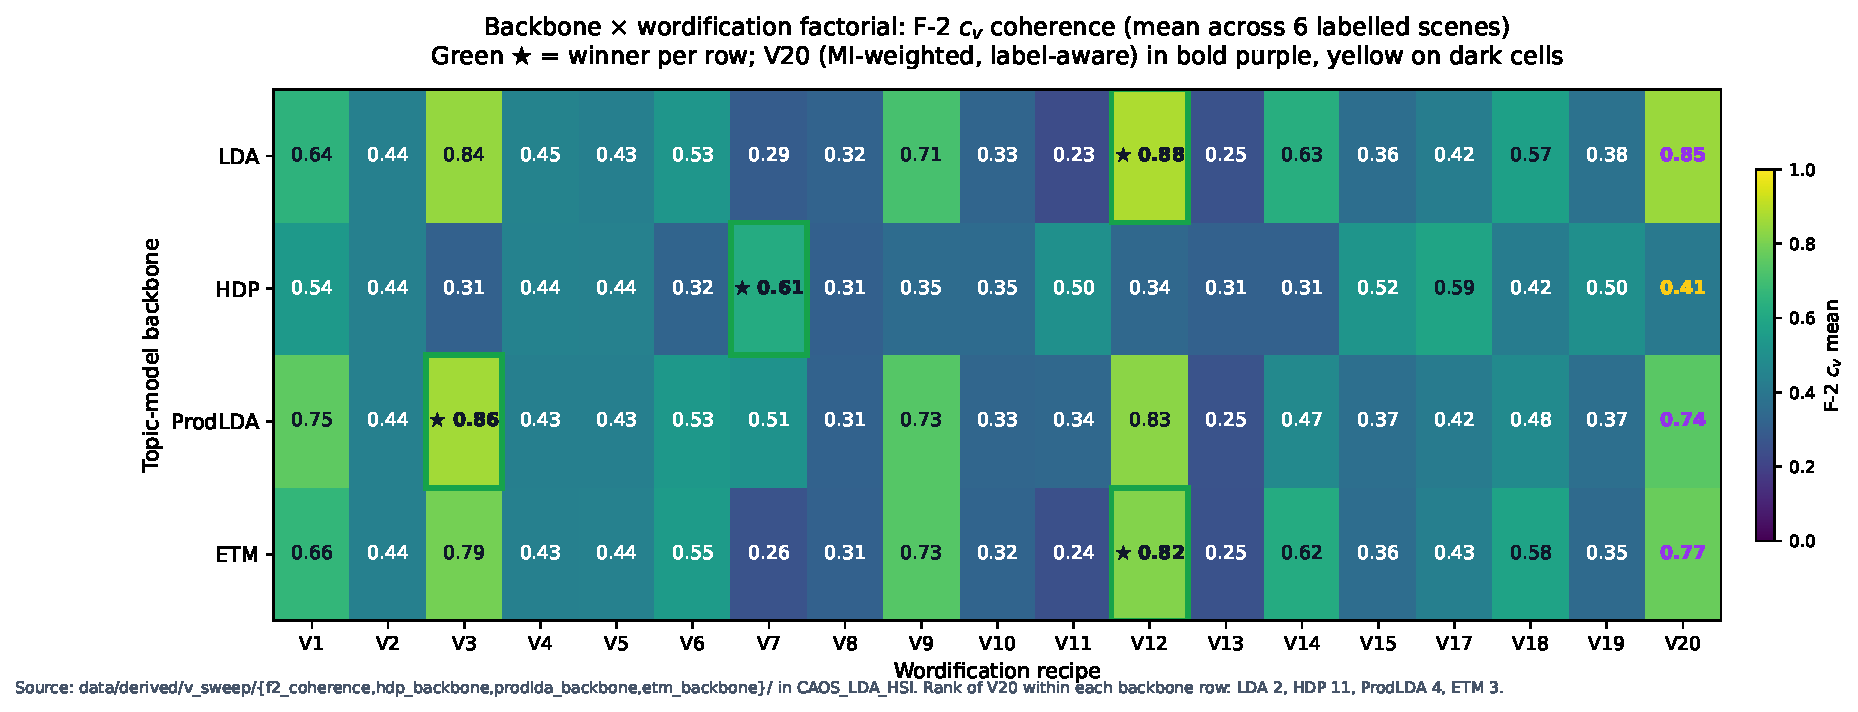
\includegraphics[width=0.99\textwidth]{p4-backbone-factorial.pdf}
\caption{F-2 $c_v$ across the $19 \times 4$ backbone factorial: a
single heatmap with one row per backbone and the recipes in index
order. $\star$ and a green border mark each row's winner (bold cell in
Table~\ref{tab:f2-factorial}); V20's value is in bold purple (yellow on
dark cells), and the footer gives V20's rank within each row. The winner moves between recipes (V12 for LDA / ETM, V3 for ProdLDA, V7
for HDP), making the recipe ranking backbone-dependent.}
\label{fig:backbone-factorial}
\end{figure*}

\subsection{Per-recipe affinity score}

We define a recipe's \emph{cross-backbone affinity score}
$\mathcal{A}(V_i)$ by \eqref{eq:affinity}: the average, over the four
backbones $\mathcal{B} = \{\mathrm{LDA}, \mathrm{HDP}, \mathrm{ProdLDA},
\mathrm{ETM}\}$, of the within-backbone min--max-normalised $c_v$ of
recipe $V_i$. $\mathcal{A} \in [0, 1]$; higher means the recipe
consistently scores near the per-backbone top across all four
backbones. Table~\ref{tab:affinity} reports $\mathcal{A}$ computed
directly from the full $19 \times 4$ cells of
Table~\ref{tab:f2-factorial}, so every recipe, including the
multi-scale V14 (continuous-wavelet tokens), the graph-Laplacian V18
and the label-aware V20, sits on one common scale
(Fig.~\ref{fig:affinity-bars}).

\begin{table}[ht]
\caption{Cross-backbone affinity scores $\mathcal{A}(V_i)$
\eqref{eq:affinity}, computed from the full $19 \times 4$ factorial of
Table~\ref{tab:f2-factorial} (min--max normalised within each backbone,
then averaged).}
\label{tab:affinity}
\centering
\small
\begin{tabular}{lc}
\toprule
Recipe & $\mathcal{A}$ \\
\midrule
V12  & 0.76 \\
V20  & 0.75 \\
V1   & 0.74 \\
V3   & 0.73 \\
V9   & 0.64 \\
V18  & 0.46 \\
V17  & 0.45 \\
V14  & 0.41 \\
V7   & 0.38 \\
V6   & 0.37 \\
V4   & 0.35 \\
V2   & 0.34 \\
V5   & 0.34 \\
V19  & 0.30 \\
V15  & 0.21 \\
V11  & 0.19 \\
V10  & 0.14 \\
V8   & 0.09 \\
V13  & 0.01 \\
\bottomrule
\end{tabular}
\end{table}

\textbf{V12 has the highest cross-backbone affinity}
($\mathcal{A} = 0.76$), with V20 ($0.75$), V1 ($0.74$) and V3 ($0.73$)
close behind. On the within-backbone normalised scale, V12, V20 and V3
score between 0.80 and 1.00 under LDA, ProdLDA and ETM, and V1
between 0.64 and 0.82; under HDP the four score 0.10 (V12), 0.32
(V20), 0.76 (V1) and 0.01 (V3). V20 is the
only \emph{label-aware} recipe in this leading group, making it the
most cross-backbone-portable label-aware recipe in the sweep and a
near-replacement for V12 / V3 when label information is available.
V3, although it only wins coherence outright under ProdLDA, remains a
top-4 affinity recipe because it is consistently strong everywhere
except HDP. \textbf{V13 (learned VQ-VAE) has the lowest affinity}
($\mathcal{A} = 0.01$), at or near the per-backbone minimum in all
four: none of the four backbones gives the reconstruction-optimal
VQ-VAE codebook coherent topics. Note that V8 scores low here
($0.09$) on \emph{coherence} affinity specifically: it is a
small-vocabulary recipe whose strength is label coupling (F-7), not
$c_v$; the F-7 factorial below ranks it very differently.

\begin{figure*}[!t]
\centering
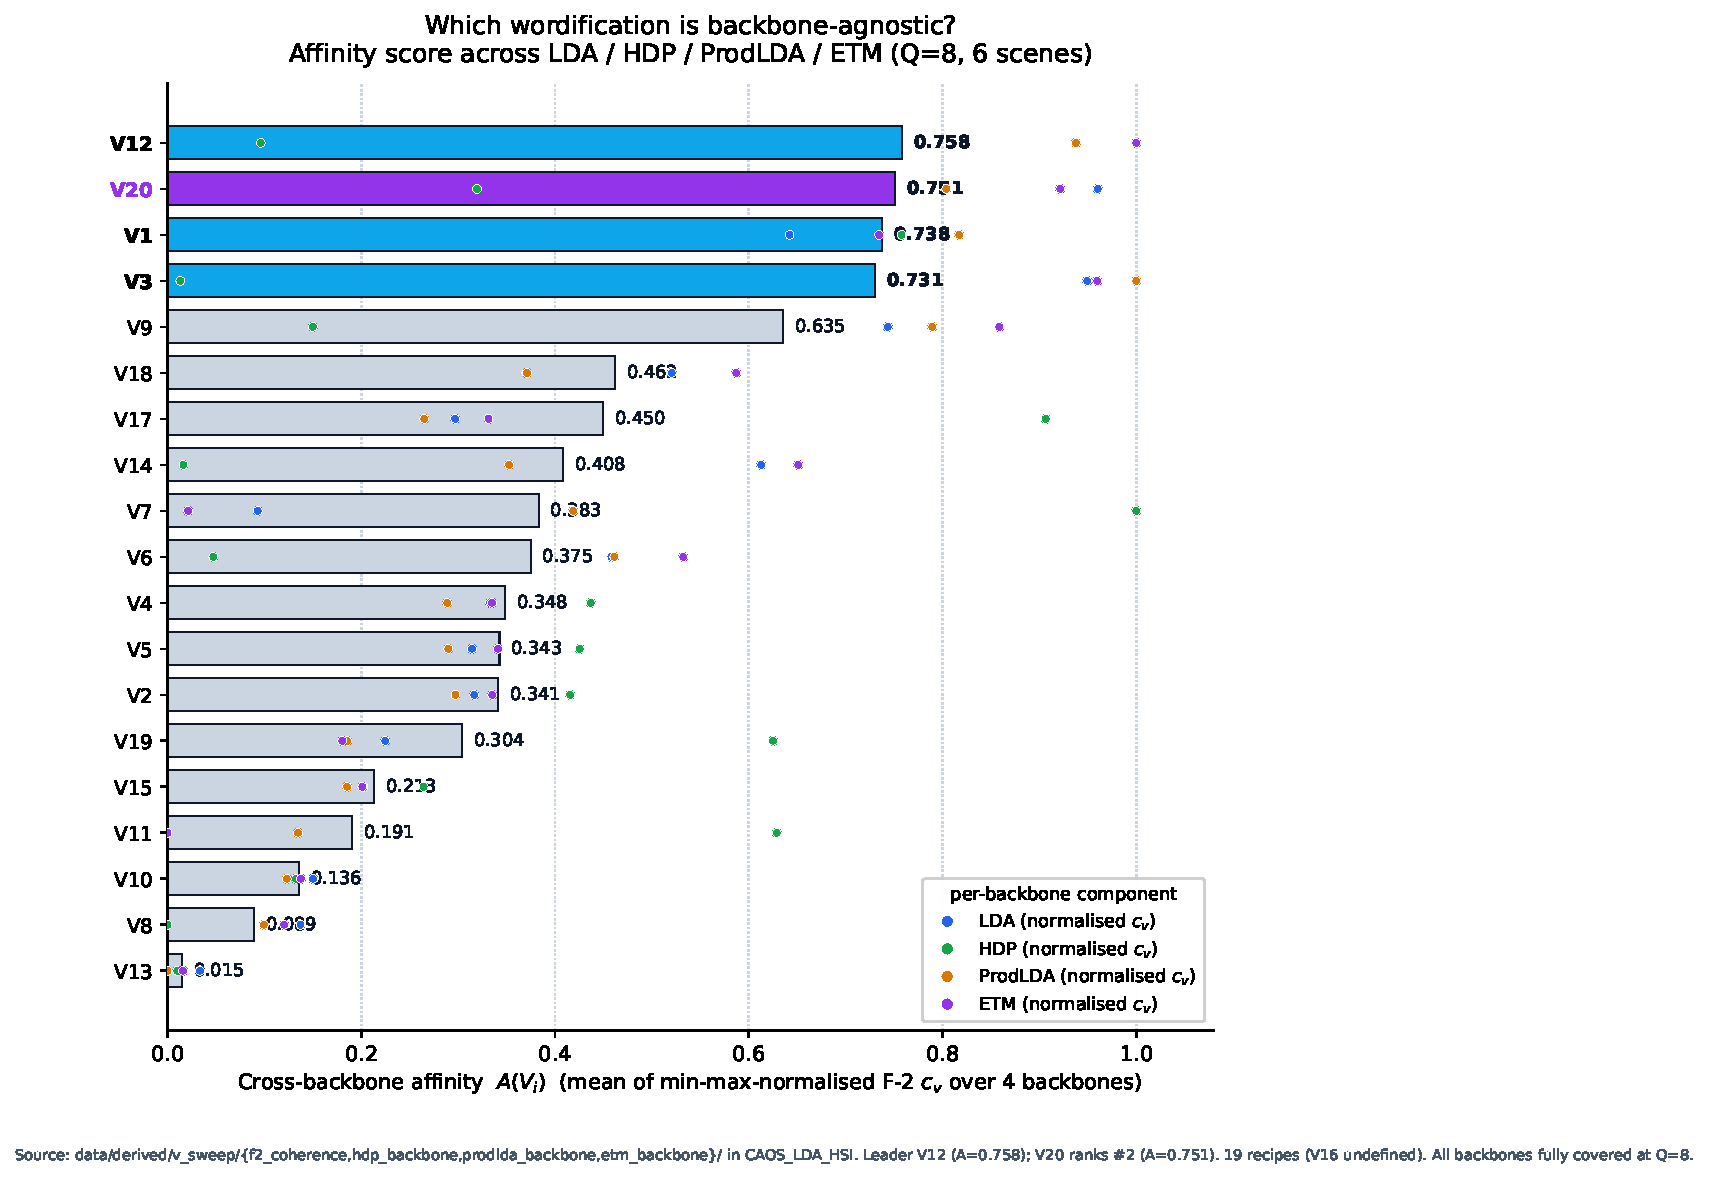
\includegraphics[width=0.70\textwidth]{p4-affinity-bars.pdf}
\caption{Cross-backbone affinity $\mathcal{A}(V_i)$ \eqref{eq:affinity}
per recipe (Table~\ref{tab:affinity}). V12 tops the ranking ($0.76$),
V20 second ($0.75$); V13 has the lowest affinity ($0.01$), at or near
the per-backbone minimum. V20 is the only label-aware recipe in the leading group.}
\label{fig:affinity-bars}
\end{figure*}

\subsection{F-7 NMI under each backbone: V8 cross-backbone leadership}
\label{subsec:f7-backbone}

We compute F-7, the label-normalised mutual
information $I(\hat Z;Y)/H(Y)$ \eqref{eq:f7} (the asymmetric uncertainty
coefficient $U(Y\mid\hat Z)$, not the symmetric NMI), between the argmax
topic per document and the
ground-truth labels for
the six labelled scenes, repeated under each backbone. The procedure
is: (1) fit the backbone via its deterministic builder (LDA, ProdLDA
and ETM with the same per-recipe K of \S\ref{sec:backbones}; HDP with
its 20-topic truncation), (2) project
each sampled labelled pixel through the fitted model to obtain the
topic mixture $\theta_d$, (3) take $z^*_d = \arg\max_k \theta_{d, k}$,
(4) compute the F-7 score $I(z^*;y)/H(y)$ of \eqref{eq:f7}. For HDP we use gensim's
\texttt{HdpModel.\_\_getitem\_\_} corpus projection; for ProdLDA and
ETM the trained encoder produces $\theta$ directly. The result is a
$19 \times 4 = 76$-cell matrix of six-scene means;
Table~\ref{tab:f7-backbone} shows the twelve recipes with the highest
four-backbone mean (48 cells). The per-scene values of all 76 cells
are in the code repository under
\path{data/derived/v_sweep/f7_topic_to_label/} (LDA) and
\path{data/derived/v_sweep/backbones_f7/} (HDP, ProdLDA, ETM); each
record carries its $K$, the number of distinct argmax topics and the
ceiling $\min(1, \log K / H(Y))$.

\begin{table}[ht]
\caption{F-7 NMI mean across the six labelled scenes for the top-12
recipes ranked by 4-backbone mean. LDA, ProdLDA and ETM share the
per-recipe $K$. Bold = per-backbone winner.}
\label{tab:f7-backbone}
\centering
\scriptsize
\setlength{\tabcolsep}{4pt}
\begin{tabular}{lccccc}
\toprule
Recipe & LDA & HDP & ProdLDA & ETM & \textbf{Mean} \\
\midrule
\textbf{V8}  (NFINDR)       & 0.463 & 0.451 & \textbf{0.328} & 0.482 & \textbf{0.431} \\
V20 (MI-weighted)           & 0.520 & 0.356 & 0.221 & \textbf{0.490} & 0.397 \\
V2  (intensity-bin)         & 0.453 & 0.347 & 0.324 & 0.456 & 0.395 \\
V12 (GMM-token)             & \textbf{0.534} & 0.220 & 0.238 & 0.488 & 0.370 \\
V3  (joint band-bin)        & 0.524 & 0.200 & 0.169 & 0.443 & 0.334 \\
V14 (CWT-Morlet)            & 0.457 & 0.220 & 0.114 & 0.430 & 0.306 \\
V11 (product quantisation)  & 0.292 & \textbf{0.571} & 0.018 & 0.329 & 0.303 \\
V15 (spectral indices)      & 0.313 & 0.438 & 0.052 & 0.297 & 0.275 \\
V19 (UMAP coord)            & 0.286 & 0.530 & 0.016 & 0.261 & 0.273 \\
V13 (VQ-VAE)                & 0.311 & 0.399 & 0.027 & 0.327 & 0.266 \\
V18 (graph-Laplacian)       & 0.428 & 0.198 & 0.080 & 0.330 & 0.259 \\
V1  (band-frequency)        & 0.455 & 0.081 & 0.091 & 0.381 & 0.252 \\
\bottomrule
\end{tabular}
\end{table}

Fig.~\ref{fig:per-scene-backbone-winners} shows the per-scene F-7 winner
under each backbone. The F-7 backbone factorial reveals
\emph{three distinct cross-backbone families}:

\paragraph{Family 1: consistently strong} V8, V20, V2. V8 is top-4
under every backbone, shares with V2 the smallest cross-backbone
standard deviation ($\sigma = 0.06$ for both) and leads at mean $0.431$
(winning outright only under ProdLDA). V2 holds that small spread at a
lower level (7th under LDA and HDP); V20 wins under ETM ($0.490$) and is
third under LDA but less cross-backbone-consistent ($\sigma = 0.12$, 6th
under HDP), and is the unique label-aware recipe here. All three have
long documents and take $K = K_{P1}$ under every fixed-$K$ backbone, so
their comparison does not depend on the topic count.

\paragraph{Family 2: HDP specialists} V11 (product quantisation) wins
HDP ($0.571$) and V19 (UMAP coordinates) is second there ($0.530$), but
both rank tenth to fifteenth under the three fixed-$K$ backbones: V11
reaches $0.292$ under LDA, $0.329$ under ETM and $0.018$ under ProdLDA,
the widest cross-backbone spread in the sweep. Both recipes emit three
or four tokens per document and take $K = 3$ under LDA, ProdLDA and ETM,
which caps F-7, bounded by $\log K / H(Y)$, at a six-scene mean of 0.46
for V11 and 0.43 for V19. LDA and ETM stay below that cap; only HDP,
which keeps up to 20 topics, exceeds it
(\S\ref{subsec:v11-mechanism}).

\paragraph{Family 3: LDA and ETM leaders} V12, V3, V14. Top-6 under
both LDA and ETM (V12 first and second, V3 second and fifth, V14 fifth
and sixth) but in the bottom half under HDP (tenth to twelfth); under
ProdLDA V12 is third, V3 fifth and V14 seventh. V12's F-7 lead under
LDA carries over to ETM, where it trails V20 by 0.002, but not to HDP,
where V11 wins, and V8 / V2 edge it out under ProdLDA.

The take-away is that the backbone factorial swap dimension matters
\emph{as much as the recipe dimension}: V11 is fourteenth under LDA
and the winner under HDP, and V12's LDA leadership carries over to ETM
but not to HDP or ProdLDA. This corroborates the P3 finding that no
recipe-backbone choice is canonical.

\subsection{Three backbone--recipe affinities}\label{sec:affinities}

The F-2 factorial (Table~\ref{tab:f2-factorial}) shows three empirical
affinities. They describe which recipe each backbone favours; the runs
do not identify why.

\textbf{LDA and ETM: dense GMM tokens.} LDA and ETM both pick V12
(GMM-token, 1600 word types from the $B \times Q$ joint vocabulary with
$B=200$, $Q=8$), with V3 and V20 close behind (LDA: V12 0.88, V20
0.85, V3 0.84; ETM: V12 0.82, V3 0.79, V20 0.77).

\textbf{HDP: sparse-event tokens.} HDP picks V7 (absorption triplets,
at most six tokens per document; 0.61), followed by V17 (0.59).

\textbf{ProdLDA: the joint (band, bin) vocabulary.} ProdLDA picks V3
(joint (band, bin) vocabulary, $B \times Q = 1600$ types; 0.86), with
V12 second (0.83).

ETM and the ProdLDA-labelled model share the $\mathcal{N}(0, I)$ prior
and the amortised encoder (\S\ref{sec:backbones}); the only implemented
difference is the decoder parameterisation. Their different winners
(V12 against V3) therefore come from the decoder parameterisation or
from optimisation, and no ablation in this study separates the two.

% =====================================================================
\begin{figure*}[!t]
\centering
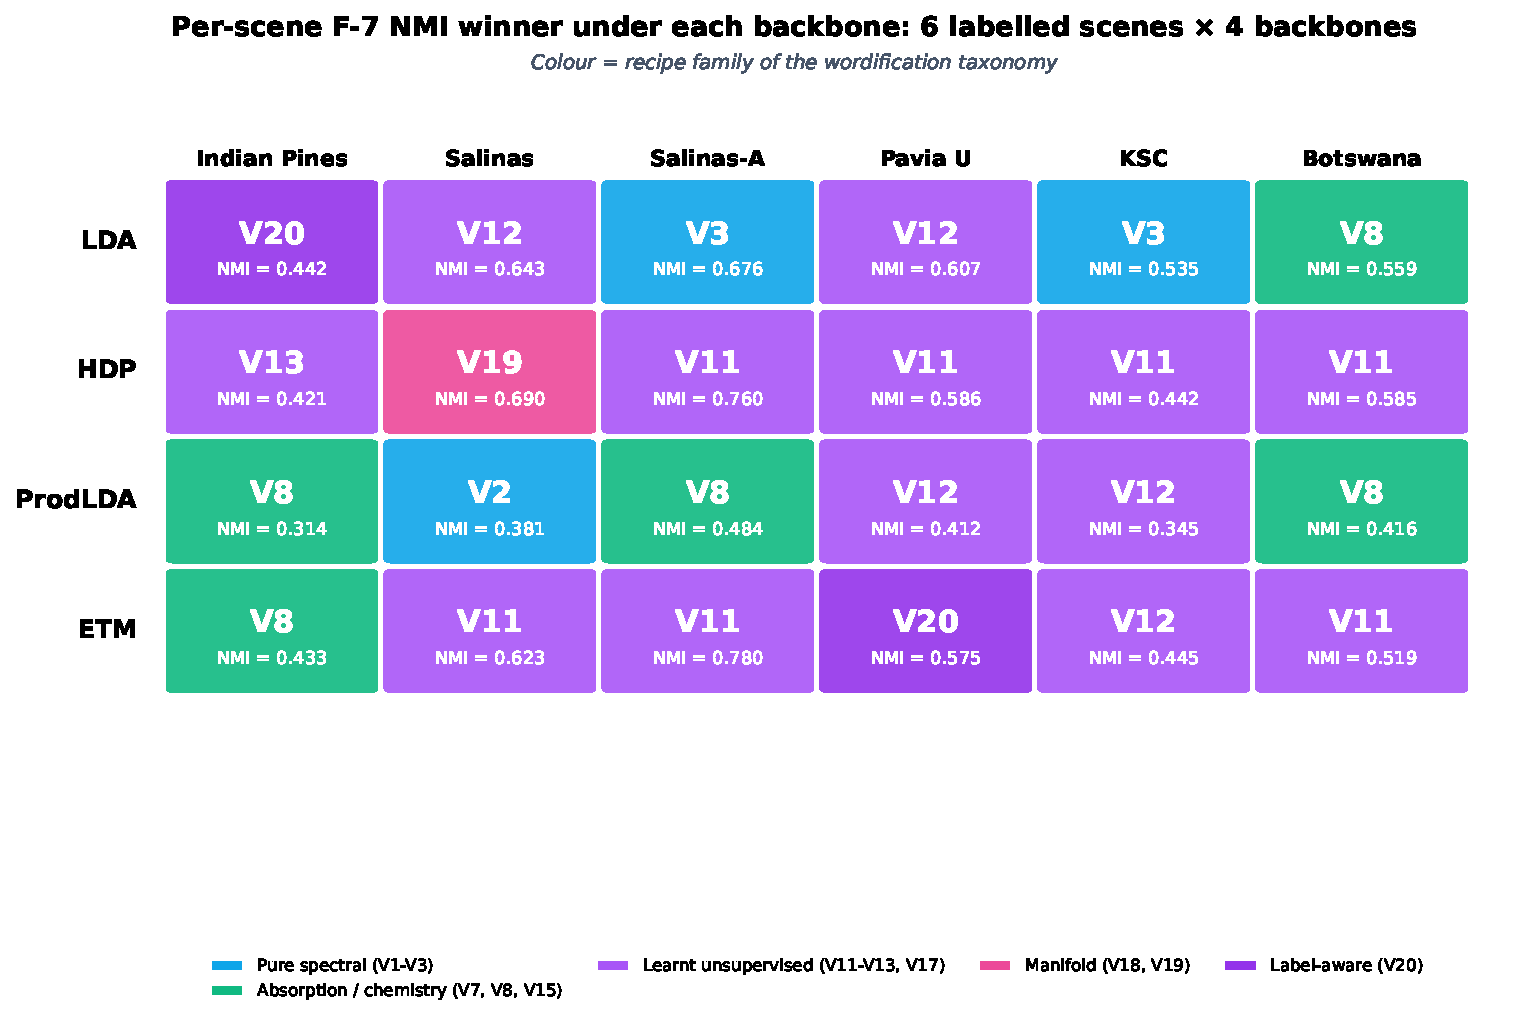
\includegraphics[width=0.95\textwidth]{p4-backbone-scene-winners.pdf}
\caption{Per-scene F-7 NMI winner under each backbone. Tile colour
encodes the winning recipe's family from the wordification taxonomy.
HDP's top winner is V11 (4/6 scenes; V13 on Indian Pines, V19 (manifold
family) on Salinas). ETM spreads its six scenes over V8 (Indian Pines,
Salinas), V20 (Pavia~U, Botswana), V2 (Salinas-A) and V12 (KSC); LDA
also spreads them over four recipes. ProdLDA favours V8 / V12 / V2.}
\label{fig:per-scene-backbone-winners}
\end{figure*}

\subsection{V11: winner under HDP, not under the fixed-K backbones}
\label{subsec:v11-mechanism}

V11 (product quantisation, $M = 4$ sub-vectors $\times$ $K_s = 8$
codewords) has a vocabulary of $M K_s = 32$ tokens, fifty times smaller
than V12's $B Q \approx 1600$; only V2 ($Q = 8$), V8 (its 6--12
endmembers), V10 and V19 ($3Q = 24$) have smaller vocabularies.
A small vocabulary fares very differently under each backbone, but
the backbones also differ in topic count, and F-7 cannot exceed
$\log K / H(Y)$. Under LDA, ProdLDA and ETM, V11's four-token
documents take $K = 3$ (\S\ref{sec:backbones}), which caps F-7 at 0.40
to 0.61 across the six scenes (six-scene mean 0.46); under LDA V11
reaches 0.77 to 0.82 of that cap on Botswana and Salinas. HDP keeps up
to 20 topics, so V11's 0.571 under HDP is out of reach of any
three-topic fit, and the HDP contrast below mixes the backbone with the
topic count; the other three backbones are compared at the same $K$:

\begin{itemize}
  \item \textbf{Under HDP}, V11 is the best recipe ($0.571$). HDP keeps
    all of its 20 truncation topics for V11 (effective number 19.9 to
    20.0 in the F-2 runs), against 1.2 to 6.2 for V12. Across the
    nineteen recipes HDP's F-7 follows the effective number of topics
    it keeps ($N_{\mathrm{eff}}$ of the F-2 runs; Spearman
    $\rho = 0.59$), and the recipes on which it keeps one or
    two topics (V1, V4, V5, V6) score F-7 near zero.
  \item \textbf{Under ETM} (embedded decoder), the topic-word
    distribution is $\beta_k = \mathrm{softmax}(\rho^{\top}\alpha_k)$
    of \eqref{eq:etm-beta}, with word embeddings
    $\rho \in \mathbb{R}^{L \times |V|}$ and topic embedding
    $\alpha_k \in \mathbb{R}^{L}$; for V11, $\rho$ is $L \times 32$.
    At $K = 3$ V11 reaches $0.329$ under ETM, 0.71 of its cap and above
    LDA's $0.292$, but it ranks tenth of the nineteen recipes; ETM's
    best recipe is V20 ($0.490$).
  \item \textbf{Under LDA}, V11 reaches only $0.292$, below the 0.46
    cap of its three topics; within that cap, topic--word distributions
    that overlap strongly over only 32 tokens may further blur the
    argmax topic, which the runs do not measure.
  \item \textbf{Under ProdLDA}, V11 collapses to $0.018$, near
    chance, although the ProdLDA-labelled model shares ETM's prior and
    encoder. The two differ only in the decoder parameterisation, so
    the collapse comes from the free topic--word matrix or from
    optimisation; the runs do not separate the two.
\end{itemize}

V19 (UMAP coords, vocab $= 24$) follows the same pattern: it is
second under HDP at 0.530, after V11 (0.571), reaches 0.286 under LDA
and 0.261 under ETM at $K = 3$, and collapses to 0.016 under ProdLDA.
The recipe--backbone choice is two-dimensional.

\section{Practical recommendation}\label{sec:recommendation}
% =====================================================================

The pair $(\text{backbone}, \text{wordification})$ is a \emph{single}
hyper-decision in LDA-on-HSI work, not two independent choices.
Reporting V12 as the best recipe is incomplete without specifying that
the result holds for LDA and ETM; reporting V3 as the best recipe is
incomplete without specifying ProdLDA.

We make three recommendations:
\begin{enumerate}
  \item Future LDA-on-HSI papers should report the
    $(\text{backbone}, \text{wordification})$ pair explicitly in
    table headers, not as separate hyperparameters.
  \item Cross-backbone affinity \eqref{eq:affinity} is a more
    informative summary than per-backbone-winner counts: it identifies
    recipes that generalise across families (V12, V20, V1, V3) versus
    those that only win in narrow regimes (V7 for HDP, V13 nowhere).
  \item V1 (band-frequency) remains a defensible \emph{reproducibility}
    canonical because of P3's F-18 result, but should not be claimed
    as a universal best on coherence in any backbone.
\end{enumerate}

% =====================================================================
\section{Limitations}\label{sec:limitations}
% =====================================================================

\begin{itemize}
  \item LDVAE-T~\cite{giannetti2025ldvaet}, a spectral-unmixing VAE with
    a Dirichlet-prior latent (an abundance/endmember model, not an
    off-the-shelf topic-model classification backbone), was considered as
    a candidate fifth backbone but has no public implementation; adapting
    it to the wordification factorial and adding its row is left to
    future work.
  \item The backbone labelled ProdLDA is the mixture-decoder form of
    \eqref{eq:prodlda-gen}; the product-of-experts ProdLDA was not run,
    and no ablation separates the decoder parameterisation from
    optimisation in the ETM--ProdLDA comparison.
  \item F-1 (Bayesian classification) is only run under LDA. Running
    F-1 under HDP / ProdLDA / ETM requires extending the topic-routed
    classifier pipeline to each backbone, which is left to future work.
  \item HDP's $K_{\text{effective}}$ is extracted as the number of
    topics holding at least $1\%$ of corpus mass under the top-level
    stick-breaking weights (the \texttt{hdp\_to\_lda} expected topic
    prevalence), feeding F-16 model-selection adequacy
    $|K_{\text{effective}}-\#\text{classes}|$; F-16 is shown in the
    interactive web application rather than tabulated here.
\end{itemize}

% =====================================================================
\section*{Data availability}
% =====================================================================

{\raggedright
Per-cell results (one JSON record per scene, recipe and backbone) are
archived in the code repository
\url{https://github.com/fsantibanezleal/CAOS_LDA_HSI} under
\path{data/derived/v_sweep/}: \path{f2_coherence/} and
\path{f7_topic_to_label/} for LDA, \path{hdp_backbone/},
\path{prodlda_backbone/} and \path{etm_backbone/} for F-2 and F-14
under the other three backbones, and \path{backbones_f7/} for their
F-7.\par}

% =====================================================================
\bibliographystyle{IEEEtran}
\bibliography{../../bibliography/refs,companion}

\end{document}
